\documentclass[tikz]{standalone}
\usepackage{pgfplots}
\usepgfplotslibrary{groupplots}
\pgfplotsset{compat=1.18}
\definecolor{utnblue}{RGB}{0, 102, 204}

\begin{document}
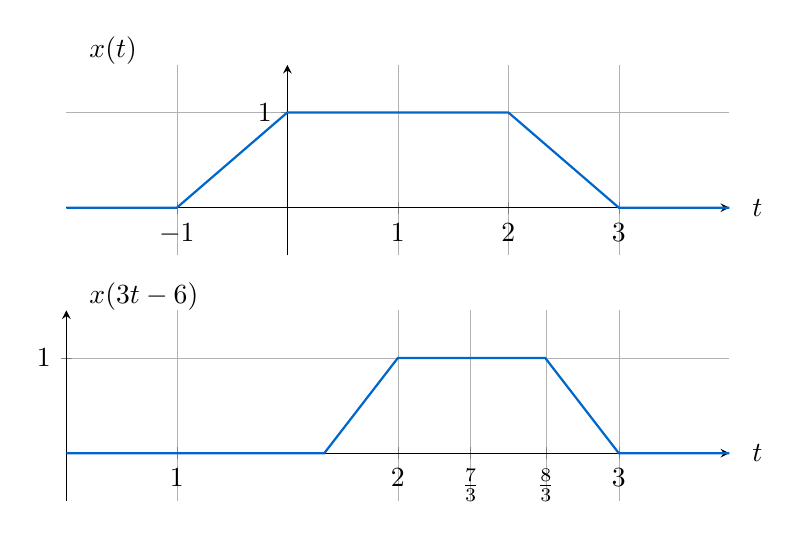
\begin{tikzpicture}
    \begin{groupplot}[
        group style={
            group size=1 by 2,
            vertical sep=0.7cm,
        },
        width=10cm,
        height=4cm,
        axis lines=middle,
        grid=both,
        grid style={line width=.1pt, draw=gray!40},
        major grid style={line width=.2pt,draw=gray!60},
        every axis plot/.append style={thick},
        every axis x label/.append style={at={(ticklabel* cs:1.02)}, anchor=west},
        every axis y label/.append style={at={(rel axis cs:0.02, 0.95)}, anchor=south west, rotate=0},
    ]
    
    % Original x(t)
    \nextgroupplot[
        xmin=-2, xmax=4, ymin=-0.5, ymax=1.5,
        xtick={-1,0,1,2,3}, ytick={0,1},
        ylabel={$x(t)$}, xlabel={$t$},
    ]
    \addplot[utnblue] coordinates {(-2,0) (-1,0) (0,1) (0,1) (2,1) (3,0) (4,0)};
    
    % x(3t-6)
    \nextgroupplot[
        xmin=0.5, xmax=3.5, ymin=-0.5, ymax=1.5,
        xtick={1,2,2.33,2.67,3},
        xticklabels={$1$,$2$,$\frac{7}{3}$,$\frac{8}{3}$,$3$},
        ytick={0,1},
        ylabel={$x(3t-6)$}, xlabel={$t$},
    ]
    \addplot[utnblue] coordinates {(0.5,0) (1.667,0) (2,1) (2,1) (2.667,1) (3,0) (3.5,0)};
    
    \end{groupplot}
\end{tikzpicture}
\end{document}
